\documentclass{standalone}
\usepackage{tikz}
\begin{document}
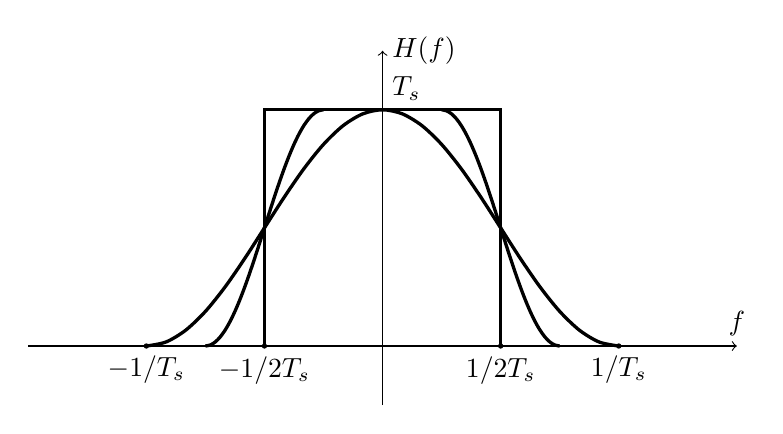
\begin{tikzpicture}[scale=3]
    \draw[->](-1.5,0)--(1.5,0)node[above]{$f$};
    \draw[->](0,-0.25)--(0,1.25)node[right]{$H(f)$};

    \draw[very thick](-0.5,0)node[below]{$-1/2T_s$}--(-0.5,1)--(0.5,1)--(0.5,0)node[below]{$1/2T_s$};
    \node[above right]at(0,1){$T_s$};
    \node[below]at(-1,0){$-1/T_s$};
    \node[below]at(1,0){$1/T_s$}; %%beta=0.5
    \draw[very thick,smooth, domain=-0.75:-0.25]plot(\x,{1/2*(1+cos(2*pi*(abs(\x)-1/4) r))});
    \draw[very thick,smooth, domain=0.25:0.75]plot(\x,{1/2*(1+cos(2*pi*(abs(\x)-1/4) r))});
    \draw[very thick,smooth, domain=-1:1]plot(\x,{1/2*(1+cos(pi*\x r))});
    \filldraw[black](-0.5,0)circle(0.25pt);
    \filldraw[black](0.5,0)circle(0.25pt);
    \filldraw[black](1,0)circle(0.25pt);
    \filldraw[black](-1,0)circle(0.25pt);
\end{tikzpicture}
\end{document}